\documentclass[a4paper]{article}

%% Language and font encodings
\usepackage[english]{babel}
\usepackage[utf8x]{inputenc}
\usepackage[T1]{fontenc}

%% Sets page size and margins
\usepackage[a4paper,top=3cm,bottom=2cm,left=3cm,right=3cm,marginparwidth=1.75cm]{geometry}

%% Useful packages
\usepackage{amsmath}
\usepackage{graphicx}
\usepackage[colorinlistoftodos]{todonotes}
\usepackage[colorlinks=true, allcolors=blue]{hyperref}

\title{Parkley Database Schema and Design}
\author{Aman Arya, Leandro Solidum}

\begin{document}
\maketitle

\section{Introduction}

This document specifies the database schema and design for Parkley, an online application that is designed to implement "parksharing" in major metropolitan areas where parking can be an issue. We describe our current database design as well as answer a few questions about the overall design choices we made while designing this database. Made as a project for INFO 340B, Fall 2017 at the University of Washington.

\section{Design Choices}

\begin{enumerate}
\item Discuss how you foresee common ways of accessing the data. \\ 

Common ways that we see of accessing the data are very similar to the three-tier architecture where the user interface is handled through either a web application or a mobile application or both. Any queries then made by the user is then moved through a web server which performs business logic (clients cannot double book a parking space, renters cannot access another renter's information, etc.). From the web server the database server is accessed which then either updates the database or queries the database for the requested information and returns it to the user in the respective medium by which they accessed the information.

Data that the user (a registered user of Parkley) could access is limited only to themselves or their respective clients or renters. A client (a registered user who currently has a booking) can access their own past transactions, current profile, and bookings but cannot access transactions of other users or clients. The only user that a client can access at the time is the renter (a registered user who has posted a driveway for rent) to see their current profile on Parkley. 

Other common ways that we imagine the database will be accessed are looking up the driveways that a renter has posted, looking at past bookings that a user has made, looking at past rentals the renter has made or finding the past bookings at a certain rental site. We ensured that these things will happen by making the Bookings entity a central entity that will allow users to look at past rentals and bookings. 

Perhaps the most common way of accessing the data will be to find the driveways around a certain user or in a certain area. To do this we have driveways linked to a city and state and have implemented a clustered index to ensure fast lookup and search for the driveways in the given city and state. 

We believe that multiple entities will want to access bookings somehow, so to account for this we added many foreign keys to the client, renters, and driveways. Bookings will also have the most information available to all parties involved so having these foreign keys will prove invaluable. 
\item Discuss what you chose to index and why.
\\ 

We chose to make clustered indexes on driveways and renters. We believed that by making clustered indexes on these entities would improve querying on these entities by the potential clients and improve overall speed and usability of the user interface. The reasoning we applied is that a user will look for renters and available driveways in a specific city or area, therefore by implementing a clustered index on both renters and driveways we can greatly improve the speed of the querying in that specific city or area the user is looking for. Though these indexes do have the disadvantage of extra space, we believe the improved user experience on the front-end will be worth this trade-off. 

In addition we decided to add a covering index to bookings because we believed that it was an entity that would be accessed often by the users. The covering index (price, city, state) we believe are attributes that the user would most likely look through and by adding this index we greatly increase the speed of our queries despite the drawback of extra space.
\item Discuss any data definitions that are not obvious.
\\

Here we will discuss the different entities that are in included our database and shown in Figure 1. 
\begin{itemize}
\item Users
\\

Users is a strong entity and is a registered user of Parkley that does not have a booking or has a rental posted currently. All renters and clients are users, but not all users are renters and/or clients. A user becomes a client once they make a booking. Once that booking ends, the client goes back to being a user. A user can become a renter by posting at least one driveway for rent. Similarly A renter becomes a user when they remove all their driveways for rent.

Their attributes reflect their user-profile that is only visible when either they are a client making a booking or they are a renter renting out their driveway and someone has made a booking to them. The client and renter entities are weak entities that are related to the entity.

\item Client
\\

Clients are a weak entity whose existence is based off the User entity. Client is separated from user because a user may or not be a client. In relation to the Booking entity, one client can make many Bookings. A client only has one booking at a time, however, clients may have had multiple bookings in the past.


Other than client-ID, a Client has a rating attribute that is determined by a Renter after the client has checked out. Renters might want to only rent out their driveways to Clients that have a minimum rating. Having this attribute will let us query to see how many clients are available with some rating.

\item Renter
\\

Renters are a weak entity who exists off the User. As discussed above, a user becomes a renter once the user posts at least one driveway for rent and returns back to being a user if they remove all driveways for rent. A renter, like the client, has a rating that is given by the client at the end of the booking period. 


Though not formulated yet, these ratings may give renters specific bonuses or move them higher in database queries when users are trying to find a driveway to rent. A renter must have at least one driveway for rent. A renter can have many driveways registered to them.

\item Booking
\\

Booking is an entity that relates clients to driveways. A client has to make a booking to park in a driveway. A client can have many bookings and a driveway can have many bookings. Booking is connected to Renter in order to calculate profits. Profits could be calculated through driveways however a chasm trap would occur in the case where a renter removes their driveway.

The spotsBooked attribute is used in conjunction with spotsAvailable from driveway to determine whether or not a driveway is available. The spotsBooked and price (from driveway) attributes determine the totalCost. The check-in, check-out and date are used to make sure the driveway is used at an available time.

\item Driveway
\\

A driveway is a registered and posted driveway available for rent by a renter. The driveway has the given attributes for price, address, and spotsAvailable that are given by the renter when they first post the driveway on Parkley. The price is defined by the renter, though we may include tools later on to help the user decide on an appropriate price for their parking spot. 

The driveway also has a rating that is given by the client. This rating can be given by proximity to major areas of interest, ease of access, cleanliness and other factors that have yet to be determined. A driveway also has spotsAvailable 
attribute which represents the number of spots available at the. This number is given by the renter. The available attribute is a boolean attribute indicating whether the driveway is currently booked or not and can be calculated by seeing the total attribute of spotsBooked in the Booking relation over spotsAvailable. 

Additionally, the driveway has a time-in and time-out that is specified by the Renter on available times that the driveway is available for a booking. We added this attribute because it is likely that the user may not want to rent out their driveway at certain times of day when they may be using it. 
\end{itemize}
\item Describe why you choose to do your schema the way you did.

We decided to split the user group into users, clients, and renters because we believed that it show the relations of the users to the company currently. A renter has a different "relationship" to the company than a client does, so we thought it would be appropriate to divide the three groups. Of course, they are all still users and connected in that sense. Also we believed it would be redundant to put multiple contact information into the database for the renters, clients and users if they are all supposed to refer to the same person. Having renters and clients be an is-a relationship in this sense solves the issue of data redundancy. 

Additionally we decided to put the renter id in the Driveway relation. We believed that this was a good idea because it could be the case that a single renter could have multiple driveways (multiple homes, big homes). Through this we would avoid duplication of Renters while still keeping the 1 to m relationship for Renters and Driveways. 

Rather than having each parking space in the driveway be its separate entity, we decided to have a driveway keep a spotsAvailable count that the renter inserts when they register the Driveway. This reduces the complexity of our Database and makes it easier to query and create for now. In the future it would be possible to have parking spaces be its own entity with all its own separate rates depending on certain features (indoor parking, access to electric-car charger, etc.).

Booking is a key entity in our Database because it links almost all the other entities together here. Bookings have to have the necessary information of all the client, renter, and driveway, so we chose this as a natural nexus of containing foreign keys to the client, renter, and driveway. Indeed, having foreign keys to the client and renter will also let the booking give the contact info of the client and renter to each other since both client and renter have user profiles. 

Instead of having a "profit" and "transaction" table in our database, which would track the profit a renter has made from till date or all transactions a client has made until now, we made several stored procedures to calculate the total profit and transactions a user or renter has made till date. Having more tables we believe will slow the database down for now, but again may be necessary further down the line. 

Finally, we decided that instead of a client making several bookings on the same driveway which would clutter the bookings table with further duplicated rows, we created a spotsBooked attribute that allows the client to book as many parking spots on the driveway as possible. Of course, to make this attribute we assume all parking spots on the driveway remain equal. Using this attribute and the number of bookings that have been made on the driveway we can calculate the availability of a driveway as well, a bit value that will indicate whether the driveway is full or not. 
\\ 
\item Have seven to ten questions that queries to your database can answer.

Here are some common queries that we believe will be made to our database.

\begin{enumerate}
\item Calculate the profit to date for the user “Aman”, “Arya”.

\begin{verbatim}
SELECT SUM(totalCost) AS Profit 
FROM Booking b, Renter r, Users u 
WHERE b.rid = r.rid AND r.uid = u.id 
AND u.fname = 'Aman' AND u.lname = 'Arya';
\end{verbatim}

\item Find the driveway for “Leandro Solidum” which makes him the most money.

\begin{verbatim}
SELECT * FROM Driveway D WHERE d.did = ( 
	SELECT TOP 1 B.did FROM Booking B 
	WHERE B.rid = ( 
		SELECT r.rid 
		FROM Renter r, Users u 
		WHERE r.uid = u.id AND u.fname = 'Leandro' AND u.lname = 'Solidum' 
	) 
	ORDER BY B.totalcost DESC 
);
\end{verbatim}

\item Apply a 10\% discount on “Aman” “Arya” last booking.

\begin{verbatim}
SELECT TOP 1 totalcost*.9 AS 'TotalCost + 10% Discount' FROM Booking B WHERE B.rid = (
		SELECT r.rid 
		FROM Renter r, Users u 
		WHERE r.uid = u.id AND u.fname = 'Aman' AND u.lname = 'Arya'
) ORDER BY dt DESC;
\end{verbatim}

\item Get the phone numbers of the client and user booking made on today’s date(2017-11-05).

\begin{verbatim}
SELECT u.phone 
FROM booking b, Client c, users u 
WHERE b.cid = c.cid AND c.uid = u.id AND b.dt = '2017-11-05'
ORDER BY b.dt;
\end{verbatim}

\item Find the price of all driveways that contain “Harrison Street” (street of Space Needle) in their address.

\begin{verbatim}
SELECT priceRate FROM Driveway d
WHERE d.address LIKE '%Harrison Street%';
\end{verbatim}

\item Find all the users who made a booking in a city that is not their own.

\begin{verbatim}
SELECT fname, lname FROM Booking B, Driveway D, Client C, Users U
WHERE B.did = D.did AND B.Cid = C.cid AND C.uid = U.id AND U.city != D.city
GROUP BY fname, lname;
\end{verbatim}

\item For each driveway find the average amount time in hours that they are booked.

\begin{verbatim}
SELECT avg(DATEDIFF(hour, checkin, checkout)) AS 'avgTimeBooked (hrs)' 
FROM Booking GROUP BY did;
\end{verbatim}

\item Find the renter with the most “available” driveway. (Driveway with the most time between time-in and time-out).

\begin{verbatim}
SELECT TOP 1 fname, lname FROM Driveway D, Renter R, Users U 
WHERE D.rid = R.rid AND R.uid = u.id 
ORDER BY DATEDIFF(hour, timein, timeout) DESC;
\end{verbatim}

\item Return how many spots are currently available in the city of Seattle.

\begin{verbatim}
Select ((SELECT SUM(spotsAvailible) FROM Driveway WHERE City = 'Seattle' 
GROUP BY City) -(SELECT SUM(spotsBooked) FROM Booking B, Driveway D WHERE B.did = d.did
AND city = 'Seattle')) AS currentlyAvailable;
\end{verbatim}

\end{enumerate}
\end{enumerate}

\begin{figure}
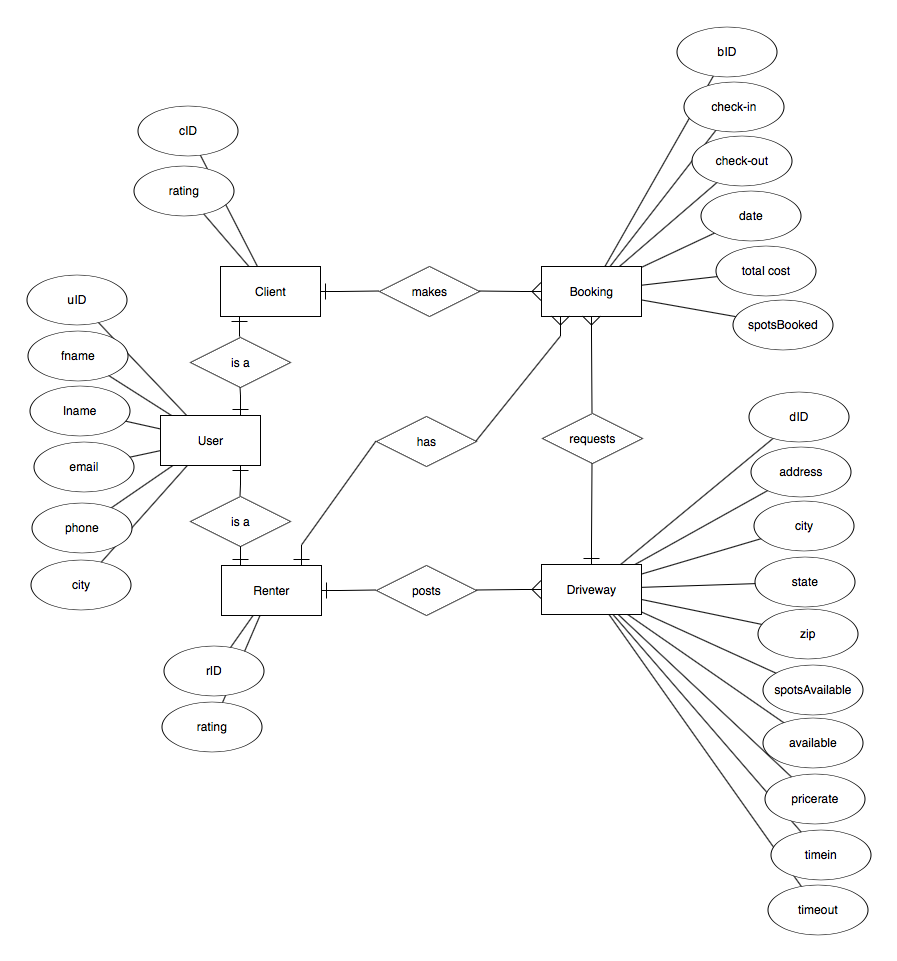
\includegraphics[scale=0.45]{parkley-erd.png}
\caption{\label{fig:erd}The ER Diagram for Parkley}
\end{figure}

\begin{figure}
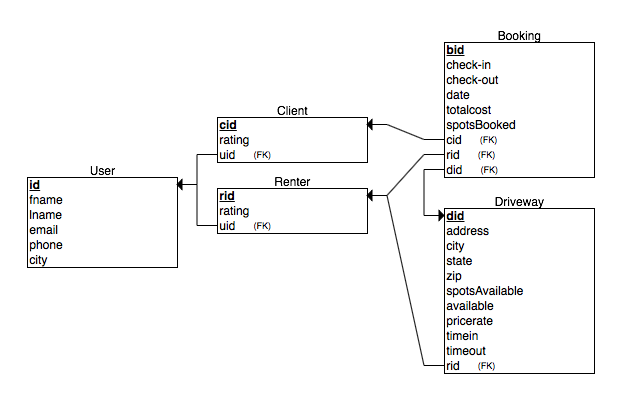
\includegraphics[scale=0.5]{parkley-schema.png}
\caption{\label{fig:schema} The Schema for Parkley}
\end{figure}

\subsection{Future Improvements}

A few future improvements that we possibly see here are the inclusion of a Parking Space relation and the further breaking down of Bookings.

Not all parking spaces are made equal. We believe that we should implement a Parking Space feature which will allow for the renter to charge different amounts for different parking spaces, instead of one amount that remains the same for all parking spaces in the driveway. Some parking spaces may be inside, in a garage, or has an electric charger. For a client to be able to use these things, they must pay extra for parking spaces that have these extra features attached to them. 

In addition, Bookings is a table that will be accessed a lot by many users of Parkley. We believe that by dividing Bookings into further parts such as having a client Booking and a renter Booking. This way we can show the relevant information to each client and renter as well as reduce the load of queries made to a single table.
\end{document}